% LaTeX Template for Project Report, Version 2.0
% (Abstracted from a Major Project Report at CSED, NIT Calicut but can be
% modified easily to use for other reports also.)
%
% Released under Creative Commons Attribution license (CC-BY)
% Info: http://creativecommons.org/licenses/by/3.0/
%
% Created by: Kartik Singhal
% BTech CSE Batch of 2009-13
% NIT Calicut
% Contact Info: kartiksinghal@gmail.com
%
% It is advisable to learn the basics of LaTeX before using this template.
% A good resource to start with is http://en.wikibooks.org/wiki/LaTeX/
%
% All template fields are marked with a pair of angular brackets e.g. <title here>
% except for the ones defining citation names in ref.tex.
%
% Empty space after chapter/section/subsection titles can be used to insert text.
%
% Just compile this file using pdflatex after making all required changes.

\documentclass[12pt,a4paper]{report}
\usepackage[pdftex]{graphicx} %for embedding images
\usepackage{url} %for proper url entries
\usepackage[bookmarks, colorlinks=false, pdfborder={0 0 0}, pdftitle={<pdf title here>}, pdfauthor={<author's name here>}, pdfsubject={<subject here>}, pdfkeywords={<keywords here>}]{hyperref} %for creating links in the pdf version and other additional pdf attributes, no effect on the printed document
%\usepackage[final]{pdfpages} %for embedding another pdf, remove if not required

\begin{document}
\renewcommand\bibname{References} %Renames "Bibliography" to "References" on ref page

%include other pages

\begin{titlepage}

\begin{center}

\textup{\bf Master Project Report} \\[0.2in]

% Title
\Large \textbf {Teakwood: An Web Framework for Handling Many-task Computing}\\[0.5in]

       \small \emph{Submitted in partial fulfillment of\\
        the requirements for the degree of}
        \vspace{.2in}

       {\bf Master in System Science} \\in\\Louisiana State University and Agricultural and Mechanical College\\ The School of Electrical Engineering and Computer Science\\
Computer Science and Engineering Division\\[0.5in]

% Submitted by
\normalsize by \\
\begin{table}[h]
\centering
\begin{tabular}{lr}\hline \\
Rui Guo \\ \\ \hline
 
%<Roll no here> & <Name here> \\
%<Roll no here> & <Name here> \\ 
%<Roll no here> & <Name here> \\ \\ \hline 
\end{tabular}
\end{table}

\vspace{.1in}
Under the guidance of\\
{\textbf{Jian Zhang}}\\[0.2in]

\vfill



%% Bottom of the page

\includegraphics[width=0.18\textwidth]{./nitc-logo}\\[0.1in]
%\Large{Department of Computer Science and Engineering}\\
%\normalsize
%\textsc{National Institute of Technology Calicut}\\
%Calicut, Kerala, India -- 673 601 \\
%\vspace{0.2cm}
\\
Fall Semester 2014

\end{center}
\end{titlepage}

\begin{center}
\bf {Preface}\\[1.0cm]
\end{center}

Four years ago, I worked for an professor


\vspace{2in}

\begin{abstract}
Using Linux commands to handle computing jobs can be a hurdle to those scientific researchers who don't have HPC related background. Teakwood provides a solution and beyond. Teakwood is a framework that migrates all the terminal typing work to a web console GUI, and provides user a total control of their jobs, data, computing resources and so on simply by clicking functional buttons. Teakwood is also an open platform that enables user to work cooperatively. Through Teakwood, user can share their models, results, and computing resources within their group and have discussions in Teakwood forum. 
\end{abstract} 


\pagenumbering{roman} %numbering before main content starts
\tableofcontents
\listoffigures

\newpage
\pagenumbering{arabic} %reset numbering to normal for the main content

\chapter{Problem Definition}

<Problem Definition here>
 %objective changed to problem definition
\chapter{Introduction}

\section{Motivation}
Four years ago, I know nothing about Linux. I then got a job to deal with HPC(High Cerformance Computing) system. Suddenly I jumped in to an UNIX environment. I found all those GUIs(Graphic User Interfaces), which I used to when I use Window OS, are gone, and I have to use Linux commands to control those machines and manage my stuff, which makes me uncomfortable and cumbersome. With the time goes by, I can work with Linux comfortably now. however, I still have the tendency to use GUI.\\I am not the only one that had such experience, In my working building, a lot of Scientists and researchers are suffering this pain. Further, cross-platform work adding them many wasteful jobs. For example, scientist A want to share a computing result for researcher B to do visualization. A uses Linux and B uses Window. What should they do? command, command, command, copy, paste, command, command ...\\Why not create a GUI platform to reduce those repeated typing work and allow them to work cooperatively?\\With all those desires, Here comes the Teakwood framework.

\section{Teakwood}
Teakwood is GUI framework that allows user to summit HPC jobs from its web console, and to have a full control of their job status. Teakwood also provides a file management systems for user to organize their job data easily. What's more, Teakwood enables user to work cooperatively by sharing their result, models and computing resources within their group. \\Teakwood migrates all the terminal typing work to Teakwood GUI, enables user to submit the HPC jobs just by simply clicking functional buttons.\\Teakwood is a web framwork, which means user can access from any type of machine as lons as the machine has a browser.

\section{Feature}
Functionally, Teakwood have the following features:\\
\\
$\bullet$ \textbf{Perfect documentation}\\
\\
Teakwood homepage provides diverse software information including installation guide, user manual, developer manual,video tutorial, etc. user can easily fetch info and grasp Teakwood soon.\\
\\
$\bullet$ \textbf{Extensible deployment}\\
\\
Teakwood is loose coupling designed. User can easily add or remove features, models or even python functions without mess the whole system.\\
\\
$\bullet$ \textbf{Neat GUI}\\
\\
A neat LSU style web console makes your work simple as Windows. Drag, push, click, that's it!\\
\\
$\bullet$ \textbf{Job monitor System}\\
\\
Job monitor system provides five labels: uploading, queued, running, finish, and Data ready to let the user monitor the job status. Job monitor system also periodically pulls the running message and displays it in the console, user can know more details about their job.\\
\\
$\bullet$ \textbf{Project management system}\\
\\
All user's project is well organized and web kept in a file server. user can compare, share, and download them as needed.\\
\\
$\bullet$ \textbf{Powerful admin}\\
\\
The powerful admin system is provided by Django itself. with tiny System configuration, use can activate their models.



 %literature survey included in this
\chapter{Teakwood System }

\section{Overview}
\section{Frontend}
\section{Backend}
\section{Data handling}
\section{Remote Configuration}

%\subsection{<Sub-section title>}
%
%\subsection{<Sub-section title>}
%some text\cite{citation-2-name-here}, some more text
%\subsection{<Sub-section title>}
%
%\subsection{<Sub-section title>}

Refer figure \ref{fig:label}.

\begin{figure}[htb]
\centering
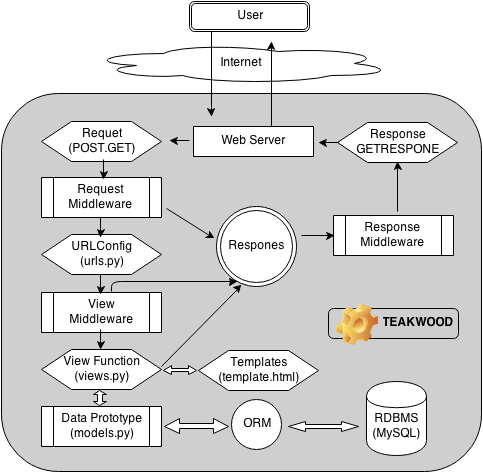
\includegraphics[scale=0.8]{./http_request_response}
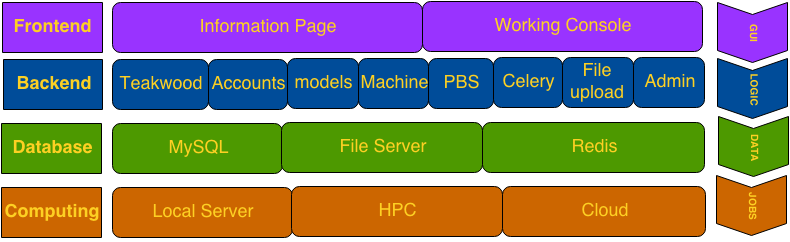
\includegraphics[scale=0.5]{./system_structure} 
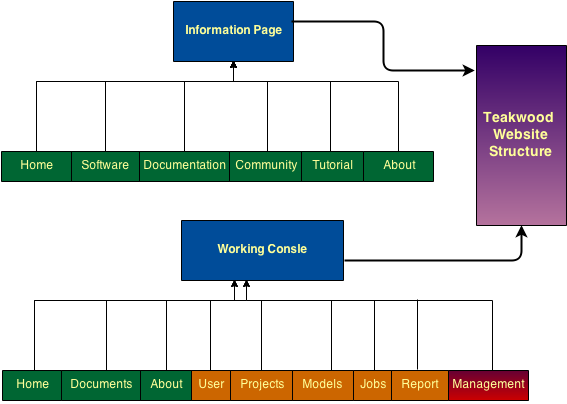
\includegraphics[scale=0.7]{./website_structure} % e.g. insert ./image for image.png in the working directory, adjust scale as necessary
\caption{<Caption here>}
\label{fig:label} % insert suitable label, this is used to refer to a fig from within the text as shown above
\end{figure}


\chapter{Future Work}

<Future work here>

\chapter{Conclusion}

The primary goal of this report is to give the reader a general overview on Teakwood. The Deep inside Logic and the Database is hard to extend.

Teakwood is written in Python, so it will be good for scientific models to 
\cleardoublepage
%\pagebreak
\phantomsection
\addcontentsline{toc}{chapter}{Acknowledgements}
\chapter*{Acknowledgments}
\vspace{1.0in}
Bootstrap CSS\\
Bootstrap JS\\
FAMFAMFAM icons\\
\newpage

\cleardoublepage
%\pagebreak
\phantomsection
\addcontentsline{toc}{chapter}{References}
\begin{thebibliography}{99}

\bibitem{citation-1-name-here}<Name of the reference here>,\ \url{<url here>}

\bibitem{citation-2-name-here}<Name of the reference here>,\ \url{<url here>}

\end{thebibliography}


\end{document}
